\documentclass{beamer}

% xcolor and define colors -------------------------
\usepackage{xcolor}

% https://www.viget.com/articles/color-contrast/
\definecolor{purple}{HTML}{5601A4}
\definecolor{navy}{HTML}{0D3D56}
\definecolor{ruby}{HTML}{9a2515}
\definecolor{alice}{HTML}{107895}
\definecolor{daisy}{HTML}{EBC944}
\definecolor{coral}{HTML}{F26D21}
\definecolor{kelly}{HTML}{829356}
\definecolor{cranberry}{HTML}{E64173}
\definecolor{jet}{HTML}{131516}
\definecolor{asher}{HTML}{555F61}
\definecolor{slate}{HTML}{314F4F}

% Mixtape Sessions
\definecolor{picton-blue}{HTML}{00b7ff}
\definecolor{violet-red}{HTML}{ff3881}
\definecolor{sun}{HTML}{ffaf18}
\definecolor{electric-violet}{HTML}{871EFF}

% Main theme colors
\definecolor{accent}{HTML}{00b7ff}
\definecolor{accent2}{HTML}{871EFF}
\definecolor{gray100}{HTML}{f3f4f6}
\definecolor{gray800}{HTML}{1F292D}


% Beamer Options -------------------------------------

% Background
\setbeamercolor{background canvas}{bg = white}

% Change text margins
\setbeamersize{text margin left = 15pt, text margin right = 15pt} 

% \alert
\setbeamercolor{alerted text}{fg = accent2}

% Frame title
\setbeamercolor{frametitle}{bg = white, fg = jet}
\setbeamercolor{framesubtitle}{bg = white, fg = accent}
\setbeamerfont{framesubtitle}{size = \small, shape = \itshape}

% Block
\setbeamercolor{block title}{fg = white, bg = accent2}
\setbeamercolor{block body}{fg = gray800, bg = gray100}

% Title page
\setbeamercolor{title}{fg = gray800}
\setbeamercolor{subtitle}{fg = accent}

%% Custom \maketitle and \titlepage
\setbeamertemplate{title page}
{
    %\begin{centering}
        \vspace{20mm}
        {\Large \usebeamerfont{title}\usebeamercolor[fg]{title}\inserttitle}\\
        {\large \itshape \usebeamerfont{subtitle}\usebeamercolor[fg]{subtitle}\insertsubtitle}\\ \vspace{10mm}
        {\insertauthor}\\
        {\color{asher}\small{\insertdate}}\\
    %\end{centering}
}

% Table of Contents
\setbeamercolor{section in toc}{fg = accent!70!jet}
\setbeamercolor{subsection in toc}{fg = jet}

% Button 
\setbeamercolor{button}{bg = accent}

% Remove navigation symbols
\setbeamertemplate{navigation symbols}{}

% Table and Figure captions
\setbeamercolor{caption}{fg=jet!70!white}
\setbeamercolor{caption name}{fg=jet}
\setbeamerfont{caption name}{shape = \itshape}

% Bullet points

%% Fix left-margins
\settowidth{\leftmargini}{\usebeamertemplate{itemize item}}
\addtolength{\leftmargini}{\labelsep}

%% enumerate item color
\setbeamercolor{enumerate item}{fg = accent}
\setbeamerfont{enumerate item}{size = \small}
\setbeamertemplate{enumerate item}{\insertenumlabel.}

%% itemize
\setbeamercolor{itemize item}{fg = accent!70!white}
\setbeamerfont{itemize item}{size = \small}
\setbeamertemplate{itemize item}[circle]

%% right arrow for subitems
\setbeamercolor{itemize subitem}{fg = accent!60!white}
\setbeamerfont{itemize subitem}{size = \small}
\setbeamertemplate{itemize subitem}{$\rightarrow$}

\setbeamertemplate{itemize subsubitem}[square]
\setbeamercolor{itemize subsubitem}{fg = jet}
\setbeamerfont{itemize subsubitem}{size = \small}

% Special characters

\usepackage{collectbox}

\makeatletter
\newcommand{\mybox}{%
    \collectbox{%
        \setlength{\fboxsep}{1pt}%
        \fbox{\BOXCONTENT}%
    }%
}
\makeatother






% Links ----------------------------------------------

\usepackage{hyperref}
\hypersetup{
  colorlinks = true,
  linkcolor = accent2,
  filecolor = accent2,
  urlcolor = accent2,
  citecolor = accent2,
}


% Line spacing --------------------------------------
\usepackage{setspace}
\setstretch{1.2}


% \begin{columns} -----------------------------------
\usepackage{multicol}


% Fonts ---------------------------------------------
% Beamer Option to use custom fonts
\usefonttheme{professionalfonts}

% \usepackage[utopia, smallerops, varg]{newtxmath}
% \usepackage{utopia}
\usepackage[sfdefault,light]{roboto}

% Small adjustments to text kerning
\usepackage{microtype}



% Remove annoying over-full box warnings -----------
\vfuzz2pt 
\hfuzz2pt


% Table of Contents with Sections
\setbeamerfont{myTOC}{series=\bfseries, size=\Large}
\AtBeginSection[]{
        \frame{
            \frametitle{Roadmap}
            \tableofcontents[current]   
        }
    }


% Tables -------------------------------------------
% Tables too big
% \begin{adjustbox}{width = 1.2\textwidth, center}
\usepackage{adjustbox}
\usepackage{array}
\usepackage{threeparttable, booktabs, adjustbox}
    
% Fix \input with tables
% \input fails when \\ is at end of external .tex file
\makeatletter
\let\input\@@input
\makeatother

% Tables too narrow
% \begin{tabularx}{\linewidth}{cols}
% col-types: X - center, L - left, R -right
% Relative scale: >{\hsize=.8\hsize}X/L/R
\usepackage{tabularx}
\newcolumntype{L}{>{\raggedright\arraybackslash}X}
\newcolumntype{R}{>{\raggedleft\arraybackslash}X}
\newcolumntype{C}{>{\centering\arraybackslash}X}

% Figures

% \imageframe{img_name} -----------------------------
% from https://github.com/mattjetwell/cousteau
\newcommand{\imageframe}[1]{%
    \begin{frame}[plain]
        \begin{tikzpicture}[remember picture, overlay]
            \node[at = (current page.center), xshift = 0cm] (cover) {%
                \includegraphics[keepaspectratio, width=\paperwidth, height=\paperheight]{#1}
            };
        \end{tikzpicture}
    \end{frame}%
}

% subfigures
\usepackage{subfigure}


% Highlight slide -----------------------------------
% \begin{transitionframe} Text \end{transitionframe}
% from paulgp's beamer tips
\newenvironment{transitionframe}{
    \setbeamercolor{background canvas}{bg=accent!40!black}
    \begin{frame}\color{accent!10!white}\LARGE\centering
}{
    \end{frame}
}


% Table Highlighting --------------------------------
% Create top-left and bottom-right markets in tabular cells with a unique matching id and these commands will outline those cells
\usepackage[beamer,customcolors]{hf-tikz}
\usetikzlibrary{calc}
\usetikzlibrary{fit,shapes.misc}

% To set the hypothesis highlighting boxes red.
\newcommand\marktopleft[1]{%
    \tikz[overlay,remember picture] 
        \node (marker-#1-a) at (0,1.5ex) {};%
}
\newcommand\markbottomright[1]{%
    \tikz[overlay,remember picture] 
        \node (marker-#1-b) at (0,0) {};%
    \tikz[accent!80!jet, ultra thick, overlay, remember picture, inner sep=4pt]
        \node[draw, rectangle, fit=(marker-#1-a.center) (marker-#1-b.center)] {};%
}

\usepackage{breqn} % Breaks lines

\usepackage{amsmath}
\usepackage{mathtools}

\usepackage{pdfpages} % \includepdf

\usepackage{listings} % R code
\usepackage{verbatim} % verbatim

% Video stuff
\usepackage{media9}

% packages for bibs and cites
\usepackage{natbib}
\usepackage{har2nat}
\newcommand{\possessivecite}[1]{\citeauthor{#1}'s \citeyearpar{#1}}
\usepackage{breakcites}
\usepackage{alltt}

% tikz
\usepackage{tikz}
\usepackage{pgfplots}
\usetikzlibrary{calc, positioning, decorations.pathreplacing, arrows.meta, intersections}
\pgfdeclarelayer{bg}
\pgfdeclarelayer{back}
\pgfdeclarelayer{fg}
\pgfsetlayers{bg,main,fg,back}
\usetikzlibrary{shapes,arrows}

% Setup math operators
\DeclareMathOperator{\E}{E} \DeclareMathOperator{\tr}{tr} \DeclareMathOperator{\se}{se} \DeclareMathOperator{\I}{I} \DeclareMathOperator{\sign}{sign} \DeclareMathOperator{\supp}{supp} \DeclareMathOperator{\plim}{plim}
\DeclareMathOperator*{\dlim}{\mathnormal{d}\mkern2mu-lim}
\newcommand\independent{\protect\mathpalette{\protect\independenT}{\perp}}
   \def\independenT#1#2{\mathrel{\rlap{$#1#2$}\mkern2mu{#1#2}}}
\newcommand*\colvec[1]{\begin{pmatrix}#1\end{pmatrix}}

\newcommand{\myurlshort}[2]{\href{#1}{\textcolor{gray}{\textsf{#2}}}}


\begin{document}

\imageframe{./lecture_includes/mixtape_ci_cover.png}


% ---- Content ----



\section{Directed Acyclic Graphs}

\begin{frame}{Graphs}

\begin{itemize}

\item Now we turn from potential outcomes modeling of causal effects to causal graphs
\item Very important area, very common to see it in computer science intersections with data science, particularly tech, and often very advanced
\item My focus is very narrow -- I am using it mainly to help us carefully reason through design elements around matching and instrumental variables

\end{itemize}

\end{frame}

\subsection{Graph notation}

\begin{frame}{Judea Pearl, 2011 Turing Award winner, drinking his first IPA}

  \begin{figure}
    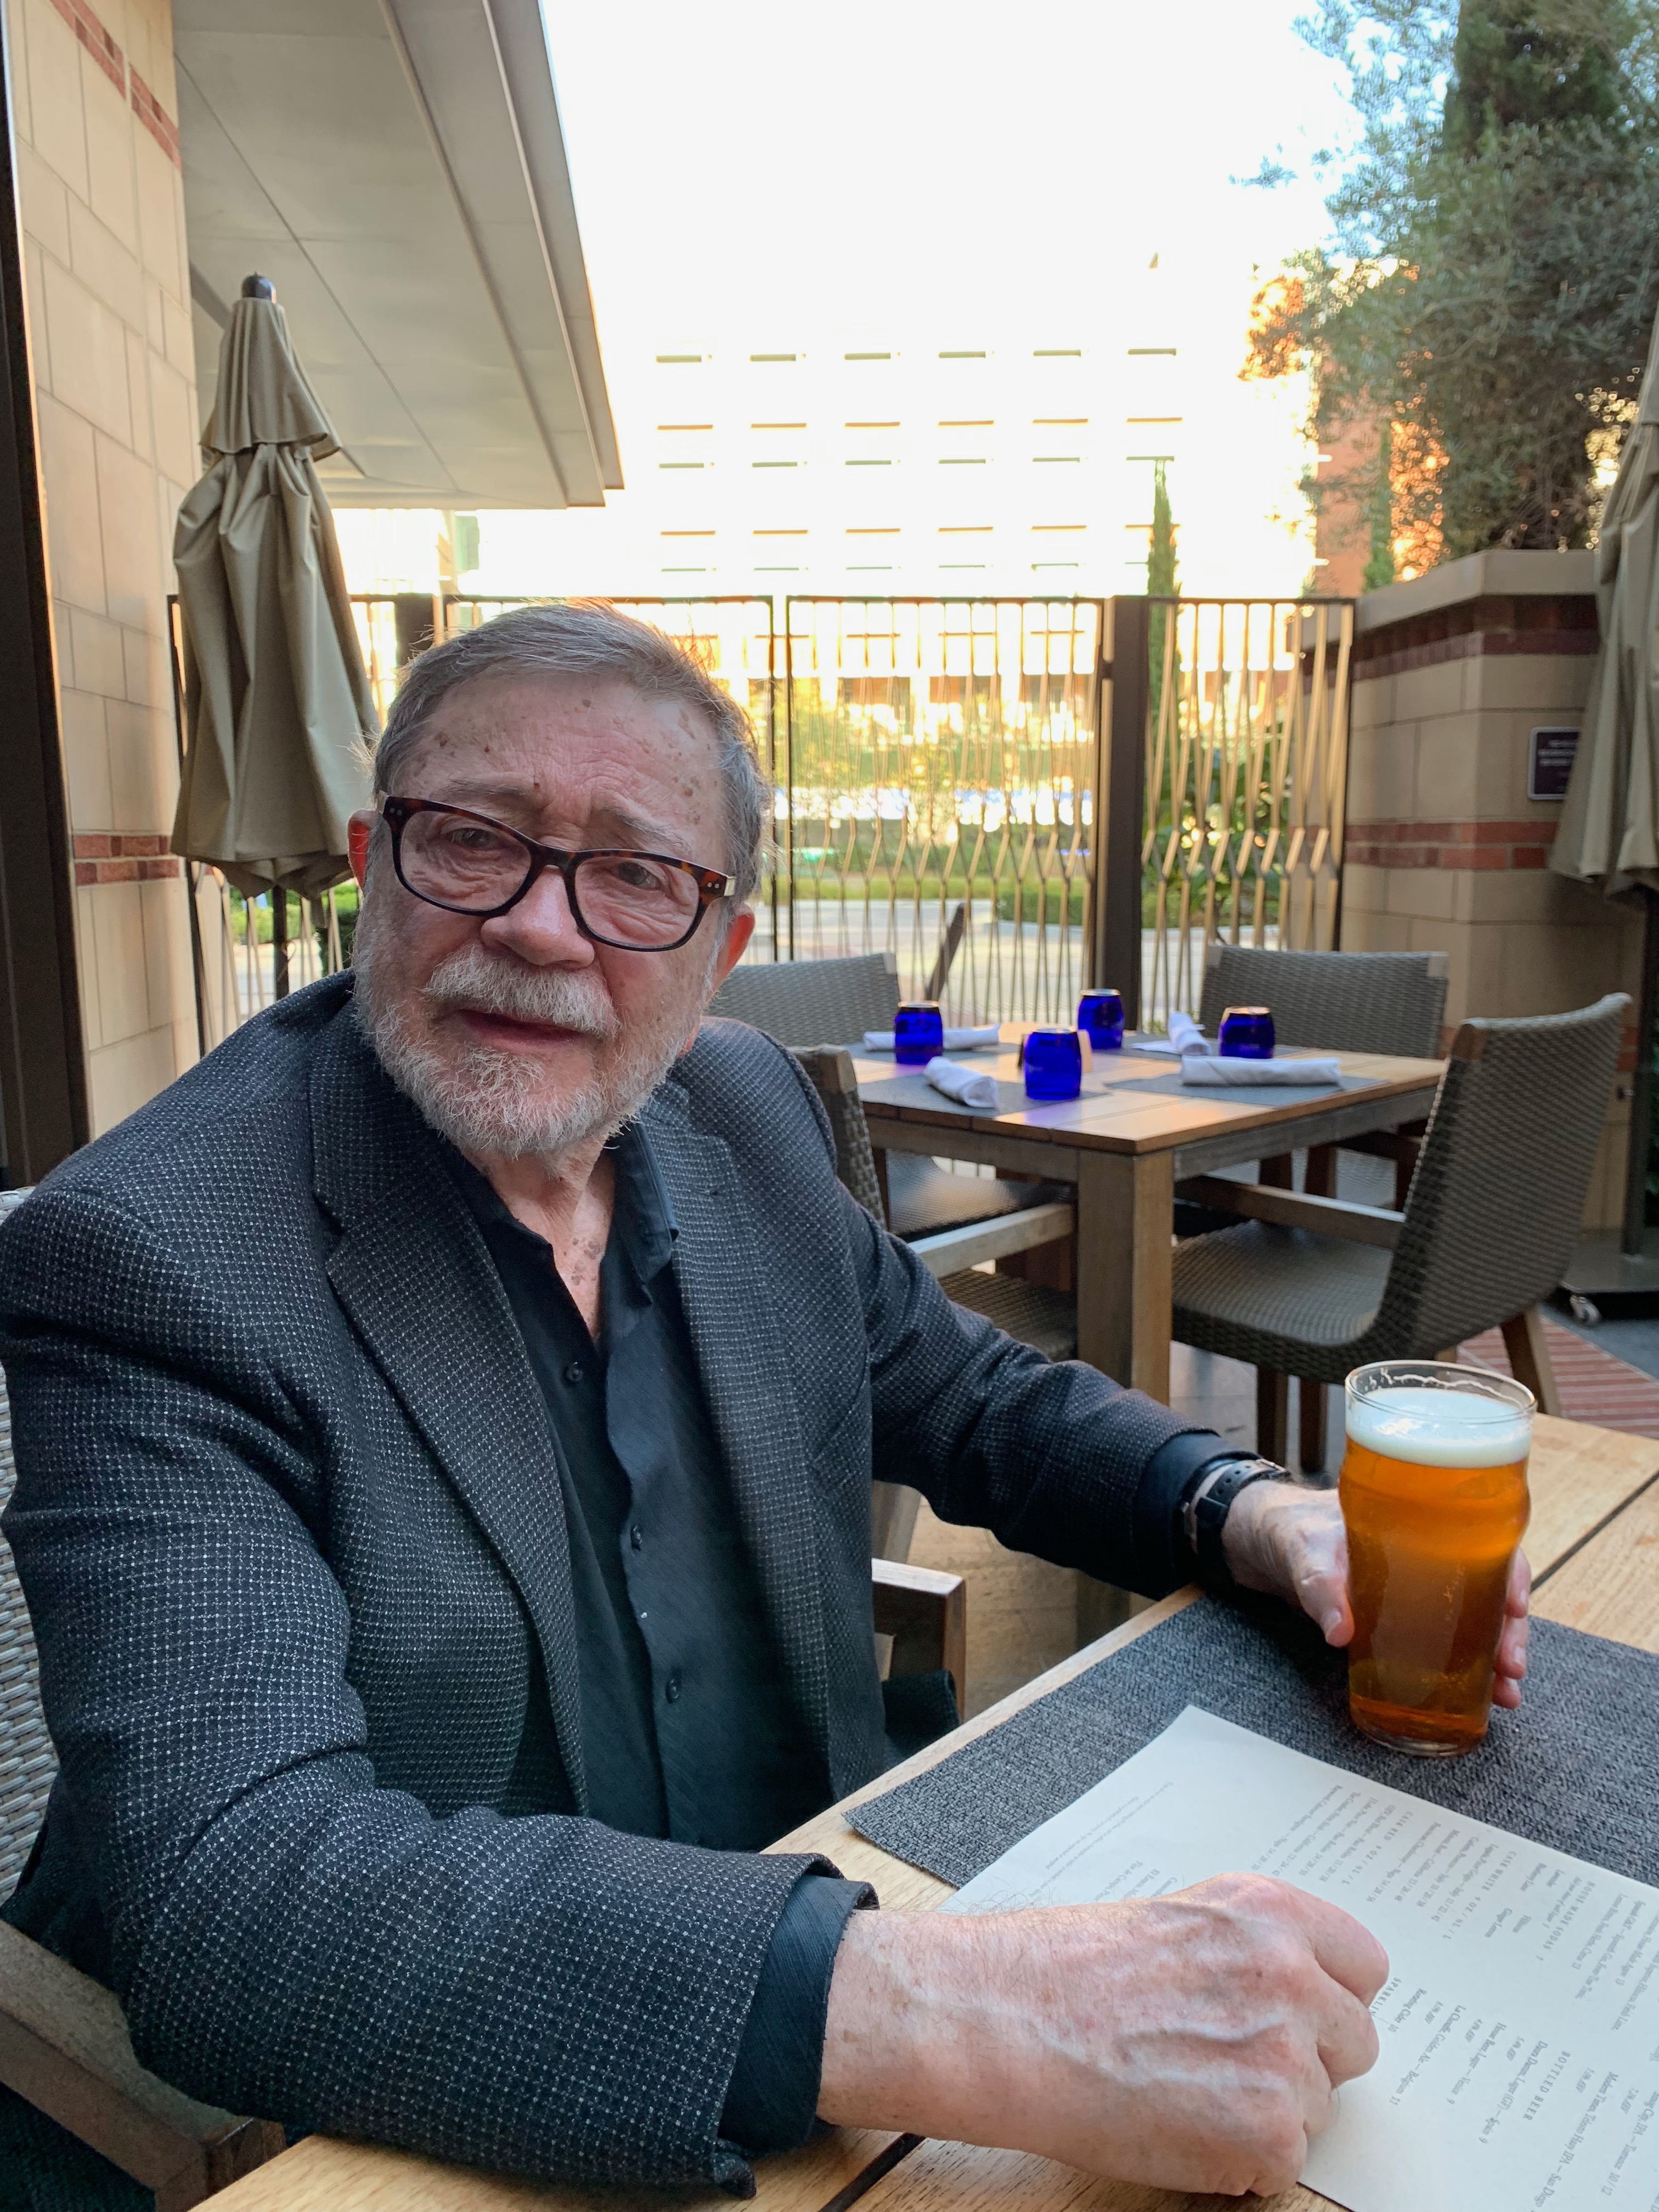
\includegraphics[scale=0.05]{./lecture_includes/pearl_ipa.jpg}
  \end{figure}

\end{frame}


\begin{frame}{Judea Pearl and DAGs}


  \begin{itemize}
    \item Judea Pearl and colleagues in Artificial Intelligence at UCLA developed DAG modeling to create a formalized causal inference methodology
    \item They make causality concepts extremely clear, they provide a map to the estimation strategy, and maybe best of all, they communicate to others what must be true about the data generating process to recover the causal effect
  \end{itemize}

\end{frame}


\begin{frame}{Further reading}

  \begin{enumerate}

    \item Pearl (2018) \underline{The Book of Why: The} \underline{New Science of Cause and Effect}, Basic Books (\emph{popular})
    \item Morgan and Winship (2014) \underline{Counterfactuals and Causal Inference: Methods and Principles} \underline{for Social Research}, Cambridge University Press, 2nd edition (\emph{excellent})
    \item Pearl, Glymour and Jewell (2016) \underline{Causal Inference In Statistics: A Primer}, Wiley Books (\emph{accessible})
    \item Pearl (2009) \underline{Causality: Models, Reasoning and Inference}, Cambridge, 2nd edition (\emph{difficult})
  \end{enumerate}

\end{frame}

\begin{frame}{Design vs. Model}

  \begin{itemize}
    \item DAGs tend to be focused more on the theory of treatment assignment in the world
    \item As such it's compatible with design-based approaches
    \item DAGs have become extremely common in industry and machine learning, so consider my review very basic comparatively as I will use them mainly to illustrate ``good vs bad controls'' as well instrumental variables
  \end{itemize}

\end{frame}



\begin{frame}{Causal model}

  \begin{itemize}
    \item The causal model is sometimes called the structural model, but for us, I prefer the former as it's less alienating
    \item It's the system of equations describing the relevant aspects of the world
    \item It necessarily is filled with causal effects associated with some particular comparative statics
    \item Consider the following diagram representing the returns to education with simplified confounders
  \end{itemize}

\end{frame}

\begin{frame}[plain]

  \begin{center}
    \begin{tikzpicture}[node distance=1.5cm]
      % nodes %
      \node[text centered] (d) {$D$};
      \node[right of = d, text centered] (y) {$Y$};
      \node[above left of = d, text centered] (i) {$I$};
      \node[left of = i, text centered] (pe) {$PE$};
      \node[below of = pe, text centered] (b) {$B$};
      % edges %
      \draw[->, line width= 1] (d) -- (y);
      \draw[->, line width= 1,] (i) -- (d);
      \draw[->, line width= 1,] (pe) -- (i);
      \draw[->, line width= 1,] (pe) -- (d);
      \draw[->, line width= 1, dashed] (b) -- (pe);
      \draw[->, line width= 1, dashed] (b) -- (d);
      \draw[->, line width= .5] (i) to [out=45,in=135, looseness=0.5] (y);
    \end{tikzpicture}
  \end{center}

  \bigskip
  \begin{itemize}
    \item $B$ is a \textbf{parent} of $PE$ and $D$
    \item $PE$ and $D$ are \textbf{descendants} of $B$
    \item There is a \textbf{direct (causal) path} from $D$ to $Y$
    \item There is a \textbf{mediated (causal) path} from $B$ to $Y$ through $D$
    \item There are six \textbf{paths} from $PE$ to $Y$ but none are direct, but some of them are different in other ways
  \end{itemize}
\end{frame}





\begin{frame}{Where do DAGs come from?}

	\begin{itemize}
	\item DAGs are meant to represent ``contemporary agreement among experts'' -- if you aren't willing to present your DAG before a room of experts, it's likely you shouldn't use it at all
	\item Your DAG should be a reasonable approximation of $D$ and $Y$ parents (confounders) and direct and indirect effects of $D$ on $Y$
	\item We get ideas for DAGs from theory, models, observation, experience, prior studies, intuition, as well as conversations with domain experts
	\end{itemize}

\end{frame}

% 	\item The DAG is a reasonable approximation of all common parents of $D$ and $Y$ (confounders) and direct relationships between $D and $Y$


\subsection{Backdoor criterion}

\begin{frame}{Unconfoundedness and the backdoor criterion}

  \begin{itemize}

    \item DAGs help us understand the source of problems in our observational (non-experimental) data that make inferring causality hard
    \item But it also can help us see a way out in some situations
    \item We will focus today on the unconfoundedness research design, which is best described in causal graphs with the concept of the \textbf{backdoor criterion}
    \item As we will see, the DAG helps you solve the problem of choosing covariates for a model to resolve selection bias, but to do so requires confidence in your DAG
  \end{itemize}

\end{frame}

\begin{frame}{Confounding}

  \begin{itemize}
    \item Confounding occurs when when the treatment and the outcomes have a common parent node as that creates spurious correlation between $D$ and $Y$

          \begin{center}
            \begin{tikzpicture}
              [node distance=1.5cm]
              % nodes %
              \node[text centered] (d) {$D$};
              \node[below right of = d, text centered] (x) {$X$};
              \node[above right of = x, text centered] (y) {$Y$};

              % edges %
              \draw[->, line width= 1] (d) -- (y);
              \draw[->, line width= 1] (x) -- (d);
              \draw[->, line width= 1] (x) -- (y);
            \end{tikzpicture}
          \end{center}

          \item The \emph{correlation} between $D$ and $Y$ is a biased measure of the average causal effect of $D$ on $Y$ because of selection bias from the confounder (ignoring for now heterogenous treatment effects bias)
  \end{itemize}
\end{frame}

\begin{frame}{Backdoor Paths}

  \begin{itemize}
    \item Confounding creates \textbf{backdoor paths} between treatment and outcome ($D\leftarrow X\rightarrow Y$) -- i.e., spurious correlations
		\begin{itemize}
		\item Not the same as a collider path ($D \rightarrow X \leftarrow Y$)
		\item and not the same as a mediator path ($D \rightarrow X \rightarrow Y$)
		\end{itemize}
    \item We can ``block'' any particular backdoor path by conditioning on variable $X$ so long as it is not a collider
    \item Once we condition on $X$, the correlation between $D$ and $Y$ estimates the causal effect of $D$ on $Y$
    \item Conditioning means calculating $E[Y|D=1,X]-E[Y|D=0,X]$ for each value of $X$ then combining (e.g., integrating) but we discuss this more later

  \end{itemize}

  \begin{center}
    \begin{tikzpicture}
      [node distance=1.5cm]
      % nodes %
      \node[text centered] (d) {$D$};
      \node[below right of = d, text centered, rectangle, draw, thin] (x) {$X$};
      \node[above right of = x, text centered] (y) {$Y$};

      % edges %
      \draw[->, line width= 1] (d) -- (y);
      \draw[->, line width= 1] (x) -- (d);
      \draw[->, line width= 1] (x) -- (y);
    \end{tikzpicture}
  \end{center}

\end{frame}



\begin{frame}{Blocked backdoor paths}

  A backdoor path is blocked if and only if:
  \begin{itemize}
    \item It contains a noncollider that has been conditioned on
    \item Or it contains a collider that has not been conditioned on
  \end{itemize}
  
  \bigskip
  
Note: A path which has a conditioned-on-collider can still be closed, but only with a noncollider-conditioned-on (we will see this later)

\end{frame}




\begin{frame}{Backdoor criterion}


  \begin{block}{Backdoor criterion}
    Conditioning on $X$ satisfies the backdoor criterion with respect to $(D,Y)$ directed path if:
    \begin{enumerate}
      \item All backdoor paths are blocked by $X$
      \item No element of $X$ is a collider 

    \end{enumerate}

    
  \end{block}
        In words: If $X$ satisfies the backdoor criterion with respect to $(D,Y)$, then controlling for or matching on $X$ identifies the causal effect of $D$ on $Y$. 

\bigskip

    And again note that a path which has a conditioned-on-collider can still be closed, but only with a noncollider-conditioned-on 

\end{frame}

\begin{frame}{What control strategy meets the backdoor criterion?}
  \begin{itemize}
    \item List all backdoor paths from $D$ to $Y$. I'll wait.

          \begin{center}
            \begin{tikzpicture}
              [node distance=1.5cm]
              % nodes %
              \node[text centered,rectangle,thin] (x1) {$X_1$};
              \node[right of = x1, text centered] (d) {$D$};
              \node[below right of = d, text centered] (x2) {$X_2$};
              \node[above right of = x2, text centered] (y) {$Y$};

              % edges %
              \draw[->, line width= .5] (x1) -- (d);
              \draw[->, line width= .5] (d) -- (y);
              \draw[->, line width= .5] (x2) -- (d);
              \draw[->, line width= .5] (x2) -- (y);
              \draw[->, line width= .5] (x1) to [out=45,in=135, looseness=0.5] (y);
            \end{tikzpicture}
          \end{center}

    \item What are the necessary and sufficient set of controls which will satisfy the backdoor criterion?
  \end{itemize}

  \framebreak




\end{frame}


\begin{frame}{What if you have an unobservable?}


  \begin{itemize}
    \item List all the backdoor paths from $D$ to $Y$.

          \begin{center}
            \begin{tikzpicture}
              [node distance=1.5cm]
              % nodes %
              \node[text centered] (u) {$U$};
              \node[right of = u, text centered] (x2) {$X_2$};
              \node[above of = x2, text centered] (x1) {$X_1$};
              \node[right of = x2, text centered] (d) {$D$};
              \node[right of = d, text centered] (y) {$Y$};

              % edges %
              \draw[->, line width= .5, dashed] (u) -- (x2);
              \draw[->, line width= .5] (x2) -- (d);
              \draw[->, line width= .5] (x1) -- (d);
              \draw[->, line width= .5] (x1) -- (y);
              \draw[->, line width= .5] (d) -- (y);
              \draw[->, line width= .5, dashed] (u) to [out=-45,in=-135, looseness=0.5] (y);
            \end{tikzpicture}
          \end{center}

    \item What are the necessary and sufficient set of controls which will satisfy the backdoor criterion?
    \item What about the unobserved variable, $U$?
  \end{itemize}

  \framebreak


\end{frame}

\begin{frame}{Multiple strategies}


  \begin{center}
    \begin{tikzpicture}
      [node distance=1.5cm, text centered]
      % nodes %
      \node[] (x3) {$X_3$};
      \node[above left of = x3,rectangle,draw,thin] (x1) {$X_1$};
      \node[below left of = x3,rectangle,draw,thin] (x2) {$X_2$};
      \node[right of = x] (d) {$D$};
      \node[right of = d] (y) {$Y$};

      % edges %
      \draw[->, line width= .5] (x1) -- (x3);
      \draw[->, line width= .5] (x2) -- (x3);
      \draw[->, line width= .5] (x1) to [out=0,in=135, looseness=0.5] (y);
      \draw[->, line width= .5] (x2) to [out=0,in=-135, looseness=0.5] (y);
      \draw[->, line width= .5] (x3) -- (d);
      \draw[->, line width= .5] (d) -- (y);
    \end{tikzpicture}

    \begin{tikzpicture}
      [node distance=1.5cm, text centered]
      % nodes %
      \node[rectangle,draw,thin] (x3) {$X_3$};
      \node[above left of = x3] (x1) {$X_1$};
      \node[below left of = x3] (x2) {$X_2$};
      \node[right of = x] (d) {$D$};
      \node[right of = d] (y) {$Y$};

      % edges %
      \draw[->, line width= .5] (x1) -- (x3);
      \draw[->, line width= .5] (x2) -- (x3);
      \draw[->, line width= .5] (x1) to [out=0,in=135, looseness=0.5] (y);
      \draw[->, line width= .5] (x2) to [out=0,in=-135, looseness=0.5] (y);
      \draw[->, line width= .5] (x3) -- (d);
      \draw[->, line width= .5] (d) -- (y);
    \end{tikzpicture}
  \end{center}

  \begin{itemize}
    \item Conditioning on the common causes, $X_1$ and $X_2$, is sufficient
    \item \dots but so is conditioning on $X_3$
  \end{itemize}
\end{frame}






\subsection{Collider bias}

\begin{frame}{Collider bias}

\begin{itemize}
\item Backdoor paths can remain open in covariate adjustment strategies through two ways:
	\begin{enumerate}
	\item You did not close the path because you did not condition on the confounder
	\item Your conditioning variable opened up a previously closed backdoor path because on that path the variable was a \textbf{collider}
	\end{enumerate}
\item Colliders are ``bad controls'' which when you control for them, \emph{create} new previously non-existent spurious correlations (not commonly discussed, even in economics)
\item This is the risk of blindly controlling for variables (``kitchen sink regressions'')
\end{itemize}

\end{frame}


\begin{frame}{Example 1: Movie stars}

  \alert{Important}: Since unconditioned colliders block back-door paths, what exactly does conditioning on a collider do? Let's illustrate with a fun example and some made-up data\\
  \begin{itemize}
    \item \underline{CNN.com} headline: Megan Fox voted worst -- but sexiest -- actress of 2009 \myurlshort{http://marquee.blogs.cnn.com/2009/12/30/megan-fox-voted-worst-but-sexiest-actress-of-2009/}{(link)}
    \item Are these two things actually negatively correlated in the world?
    \item Assume talent and beauty are independent, but each causes someone to become a movie star.  What's the correlation between talent and beauty for a sample of movie stars compared to the population as a whole (stars and non-stars)?
  \end{itemize}

\end{frame}


\begin{frame}{Movie star DAG}

Imagine casting directors pick movie stars based on talent and beauty

  \begin{center}
    \begin{tikzpicture}
      [node distance=2cm, text centered]

      %nodes
      \node[text centered,draw,rectangle,thin] (x) {Movie Star};
      \node[below left of = x] (u1) {$Talent$};
      \node[below right of = x] (u2) {$Beauty$};

      % edges %
      \draw[->, line width= 2] (u1) -- (x);
      \draw[->, line width= 2] (u2) -- (x);
    \end{tikzpicture}
  \end{center}

Talent and beauty can become correlated even though they are independent


\end{frame}

\begin{frame}[shrink=20,plain]

  \begin{figure}
    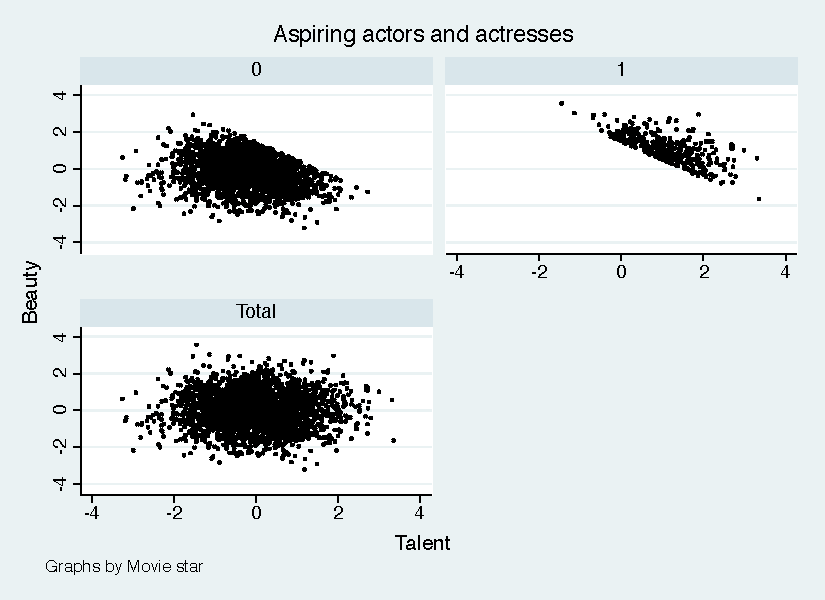
\includegraphics[height=9cm]{./lecture_includes/beauty_collider.pdf}
    \caption{Top left figure: Non-star sample scatter plot of beauty (vertical axis) and talent (horizontal axis). Top right right figure: Star sample scatter plot of beauty and talent.  Bottom left figure: Entire (stars and non-stars combined) sample scatter plot of beauty and talent.}
  \end{figure}
\end{frame}

\begin{frame}{Sample selection?}

\begin{itemize}
\item Notice that this is clear when we are focused on sample selection
\item But even a regression that included ``star'' would create the issue:$$talent_i = \alpha + \delta beauty_i + \beta star_i + \varepsilon_i$$
\item It's not just sample selection 
\end{itemize}

\end{frame}


\begin{frame}{Example 2: Discrimination}

  \begin{itemize}
    \item Let's look at another example: very common for think tanks and journalists to say that the gender gap in earnings disappears once you control for occupation.
    \item But what if occupation is a collider, which it could be in a model with occupational sorting
    \item Then controlling for occupation in a wage regression searching for discrimination can lead to all kinds of crazy results \emph{even in a simulation where we explicitly design there to be discrimination}
  \end{itemize}

\end{frame}

\begin{frame}{DAG}

  \begin{center}
    \begin{tikzpicture}
      [node distance=1.5cm]
      % nodes %
      \node[text centered] (f) {$F$};
      \node[above right of = f, text centered] (d) {$d$};
      \node[right of = f] (y) {$y$};
      \node[below  of = f, text centered] (o) {$o$};
      \node[right of = o, text centered] (a) {$A$};

      % edges %
      \draw[->, line width= 1] (f) -- (d);
      \draw[->, line width= 1] (d) -- (o);
      \draw[->, line width= 1, dashed] (a) -- (o);

      \draw[->, line width= 1] (d) -- (y);
      \draw[->, line width= 1] (o) -- (y);
      \draw[->, line width= 1, dashed] (a) -- (y);

    \end{tikzpicture}
  \end{center}

  $F$ is female, $d$ is discrimination, $o$ is occupation, $y$ is earnings and $A$ is ability. Dashed lines mean the variable cannot be observed. Note, by design, being a female has no effect on earnings or occupation, and has no relationship with ability. So earnings is coming through discrimination, occupation, and ability.

\end{frame}


\begin{frame}[plain]

  \begin{center}
    \begin{tikzpicture}
      [node distance=1.5cm]
      % nodes %
      \node[text centered] (f) {$F$};
      \node[above right of = f, text centered] (d) {$d$};
      \node[right of = f] (y) {$y$};
      \node[below  of = f, text centered] (o) {$o$};
      \node[right of = o, text centered] (a) {$A$};

      % edges %
      \draw[->, line width= 1] (f) -- (d);
      \draw[->, line width= 1] (d) -- (o);
      \draw[->, line width= 1, dashed] (a) -- (o);

      \draw[->, line width= 1] (d) -- (y);
      \draw[->, line width= 1] (o) -- (y);
      \draw[->, line width= 1, dashed] (a) -- (y);

    \end{tikzpicture}
  \end{center}


  Mediation and Backdoor paths

  \begin{enumerate}

    \item $d$ $\rightarrow o \rightarrow y$
    \item $d$ $\rightarrow o \leftarrow A \rightarrow y$
  \end{enumerate}

\end{frame}


\begin{frame}[plain, shrink=20]

  \begin{table}[htbp]\centering
    \scriptsize
    \caption{Regressions illustrating collider bias with simulated gender disparity}
    \begin{center}
      \begin{tabular}{l*{3}{c}}
        \toprule
        \multicolumn{1}{l}{Covariates: }&
        \multicolumn{1}{c}{\textbf{Unbiased combined effect}}&
        \multicolumn{1}{c}{\textbf{Biased }}&
        \multicolumn{1}{c}{\textbf{Unbiased wage effect only}}\\
        \midrule
        Female                     & -3.074*** & 0.601*** & -0.994*** \\
                                   & (0.000)   & (0.000)  & (0.000)   \\
        Occupation                 &           & 1.793*** & 0.991***  \\
                                   &           & (0.000)  & (0.000)   \\
        Ability                    &           &          & 2.017***  \\
                                   &           &          & (0.000)   \\
        \\
        \midrule
        N                          & 10,000    & 10,000   & 10,000    \\
        Mean of dependent variable & 0.45      & 0.45     & 0.45      \\
        \bottomrule
      \end{tabular}
    \end{center}
  \end{table}

  \begin{itemize}
    \item Recall we designed there to be a discrimination coefficient of -1
    \item If we do not control for occupation, then we get the combined effect of $d \rightarrow o \rightarrow y$ and $d  \rightarrow y$
    \item Because it seems intuitive to control for occupation, notice column 2 - the sign flips!
    \item We are only able to isolate the direct causal effect by conditioning on ability and occupation, but ability is unobserved
  \end{itemize}

\end{frame}

\begin{frame}[allowframebreaks,plain]

  \begin{itemize}
    \item \textbf{Colliders can be outcomes (and often those are the ones)}
          \begin{itemize}
            \item There is only one backdoor path from $D$ to $Y$

                  \begin{center}
                    \begin{tikzpicture}
                      [node distance=1.5cm]
                      % nodes %
                      \node[text centered,draw,rectangle,thin] (x1) {$X_1$};
                      \node[right of = x1, text centered] (d) {$D$};
                      \node[below right of = d, text centered] (x2) {$X_2$};
                      \node[above right of = x2, text centered] (y) {$Y$};

                      % edges %
                      \draw[->, line width= .5] (x1) -- (d);
                      \draw[->, line width= .5] (d) -- (y);
                      \draw[->, line width= .5] (d) -- (x2);
                      \draw[->, line width= .5] (y) -- (x2);
                      \draw[->, line width= .5] (x1) to [out=45,in=135, looseness=0.5] (y);
                    \end{tikzpicture}
                  \end{center}
                  

            \item Conditioning on $X_1$ blocks the backdoor path


            \item But what if we also condition on $X_2$?

                  \begin{center}
                    \begin{tikzpicture}
                      [node distance=1.5cm]
                      % nodes %
                      \node[text centered,draw,rectangle,thin] (x1) {$X_1$};
                      \node[right of = x1, text centered] (d) {$D$};
                      \node[below right of = d, draw, rectangle, text centered] (x2) {$X_2$};
                      \node[above right of = x2, text centered] (y) {$Y$};

                      % edges %
                      \draw[->, line width= .5] (x1) -- (d);
                      \draw[->, line width= .5] (d) -- (y);
                      \draw[->, line width= .5] (d) -- (x2);
                      \draw[->, line width= .5] (y) -- (x2);
                      \draw[->, line width= .5] (x1) to [out=45,in=135, looseness=0.5] (y);
                    \end{tikzpicture}
                  \end{center}

            \item Conditioning on $X_2$ opens up a new path, creating new spurious correlations between $D$ and $Y$ 
          \end{itemize}

          \framebreak


    \item \textbf{Colliders could be pre-treatment covariates (called M-bias because it looks like an M)}
          \begin{itemize}
            \item Name the backdoor paths.  Is it open or closed?

                  \begin{center}
                    \begin{tikzpicture}
                      [node distance=1.5cm, text centered]
                      % nodes %
                      \node[] (x) {$X$};
                      \node[above left of = x] (u1) {$U_1$};
                      \node[below left of = x] (u2) {$U_2$};
                      \node[right of = x] (d) {$D$};
                      \node[right of = d] (y) {$Y$};

                      % edges %
                      \draw[->, line width= .5, dashed] (u1) -- (x);
                      \draw[->, line width= .5, dashed] (u2) -- (x);
                      \draw[->, line width= .5, dashed] (u1) to [out=0,in=135, looseness=0.5] (y);
                      \draw[->, line width= .5, dashed] (u2) to [out=0,in=-135, looseness=0.5] (d);
                      \draw[->, line width= .5] (d) -- (y);
                    \end{tikzpicture}
                  \end{center}

            \item But what if we condition on $X$?

                  \begin{center}
                    \begin{tikzpicture}
                      [node distance=1.5cm, text centered]
                      % nodes %
                      \node[text centered,draw,rectangle,thin] (x) {$X$};
                      \node[above left of = x] (u1) {$U_1$};
                      \node[below left of = x] (u2) {$U_2$};
                      \node[right of = x] (d) {$D$};
                      \node[right of = d] (y) {$Y$};

                      % edges %
                      \draw[->, line width= .5, dashed] (u1) -- (x);
                      \draw[->, line width= .5, dashed] (u2) -- (x);
                      \draw[->, line width= .5, dashed] (u1) to [out=0,in=135, looseness=0.5] (y);
                      \draw[->, line width= .5, dashed] (u2) to [out=0,in=-135, looseness=0.5] (d);
                      \draw[->, line width= .5] (d) -- (y);
                    \end{tikzpicture}
                  \end{center}


          \end{itemize}
  \end{itemize}
  \framebreak


\end{frame}


\begin{frame}{Testing the Validity of the DAG}

  \begin{itemize}
    \item The DAG makes testable predictions
    \item Conditional on $D$ and $I$, parental education ($PE$) should no longer be correlated with $Y$
    \item Can be hard to figure this out by hand, but software can help (e.g., Daggity.net is browser based, Causal Fusion is more advanced)
    \item Causal algorithms tend to be DAG based and are becoming popular in industry 
  \end{itemize}

  \begin{center}
    \begin{tikzpicture}[node distance=1.5cm]
      % nodes %
      \node[text centered] (d) {$D$};
      \node[right of = d, text centered] (y) {$Y$};
      \node[above left of = d, text centered] (i) {$I$};
      \node[left of = i, text centered] (pe) {$PE$};
      \node[below of = pe, text centered] (b) {$B$};
      % edges %
      \draw[->, line width= 1] (d) -- (y);
      \draw[->, line width= 1,] (i) -- (d);
      \draw[->, line width= 1,] (pe) -- (i);
      \draw[->, line width= 1,] (pe) -- (d);
      \draw[->, line width= 1, dashed] (b) -- (pe);
      \draw[->, line width= 1, dashed] (b) -- (d);
      \draw[->, line width= .5] (i) to [out=45,in=135, looseness=0.5] (y);
    \end{tikzpicture}
  \end{center}

\end{frame}




\subsection{Concluding remarks}


\begin{frame}{Summarizing all of this}

  \begin{itemize}
    \item Your dataset will not come with a codebook flagging some variables as ``confounders'', ``mechanisms'' and ``colliders'' because those terms are always context specific
    \item Except for some unique situations that aren't generally applicable, you also don't always know statistically you have an omitted variable bias problem; but both of these are fatal for any application
    \item You only know to do what you're doing based on \emph{knowledge about data generating process}.
    \item All identification must be guided by theory, experience, observation, common sense and knowledge of institutions
    \item DAGs absorb that information and can be then used to write out the explicit identifying model
  \end{itemize}

\end{frame}





\end{document}

\begin{frame}{DAGs are not panacea}

  \begin{itemize}
    \item DAGs cannot handle, though, reverse causality or simultaneity
    \item So there are limitations.  ``All models are wrong but some are useful''
    \item But I think they are helpful and while not \emph{necessary}, showcase what is necessary -- assumptions
    \item Heckman (1979) can maybe provide some justification at times
  \end{itemize}

\end{frame}

\subsection{Front door criterion}

\begin{frame}{Research design \#2: front door criterion}

  \begin{itemize}
    \item Confounding creates major issues for us, but if we can observe the confounders, then we can use the backdoor criterion (``selection on observables'') to identify causal effects
    \item What about \textbf{unobserved confounding}?  It depends on the DAG
    \item One particular DAG structure that is not widely known outside of Pearl circles is the front door criterion
    \item Bears some topical resemblance to instrumental variables, but it is nonetheless very different and when available to you the elements can be used to trace out causal effects
  \end{itemize}

\end{frame}

\begin{frame}{Mechanisms}

  \begin{itemize}
    \item Rarely does an intervention operate directly on an outcome; oftentimes it operates on the outcome via a ``mechanism''
          \begin{itemize}
            \item Example: Parental substance abuse causes foster care removals through child abuse and neglect
          \end{itemize}
    \item The presence of mechanisms, it turns out, is valuable because of their policy relevance, but also because we can use them \emph{sometimes} for identification
  \end{itemize}

\end{frame}

\begin{frame}{Frontdoor DAG}

  \begin{center}
    \begin{tikzpicture}[node distance=1.5cm]
      % nodes %
      \node[text centered] (d) {$D$};
      \node[right of = d, text centered] (m) {$M$};
      \node[right of = m, text centered] (y) {$Y$};
      \node[below of = m, text centered] (u) {$U$};
      % edges %
      \draw[->, line width= 1] (d) -- (m);
      \draw[->, line width= 1] (m) -- (y);
      \draw[->, line width= 1, dashed] (u) -- (d);
      \draw[->, line width= 1, dashed] (u) -- (y);
    \end{tikzpicture}
  \end{center}

  \begin{itemize}
    \item We cannot close $D \leftarrow U \rightarrow Y$ because $U$ is not observed and thus simple contrasts are biased estimates of treatment effects
    \item Pearl (2009) showed that this DAG actually does allow us to recover the effect of $D$ on $Y$, though -- just not via the backdoor criterion
  \end{itemize}

\end{frame}

\begin{frame}{Front door criterion}

  \begin{quote}
    If one or more unblocked back door paths connect a causal variable to an outcome variable, the causal effect is identified by conditioning on a set of observed variables $M$ that make up the identifying mechanism if and only if: 1) the variables in $M$ intercept all directed paths from the causal variable to the outcome (``exhaustiveness''); 2) No unblocked back-door paths connecting the causal variable to the variables in the set $M$ and all back door paths from the variables in $M$ to the outcome can be blocked by conditioning on $D$ (``isolation'')
  \end{quote}

\end{frame}

\begin{frame}{Exhaustiveness}

  \begin{center}
    \begin{tikzpicture}[node distance=1.5cm]
      % nodes %
      \node[text centered] (d) {$D$};
      \node[right of = d, text centered] (m) {$M$};
      \node[right of = m, text centered] (y) {$Y$};
      \node[below of = m, text centered] (u) {$U$};
      % edges %
      \draw[->, line width= 1] (d) -- (m);
      \draw[->, line width= 1] (m) -- (y);
      \draw[->, line width= 1, dashed] (u) -- (d);
      \draw[->, line width= 1, dashed] (u) -- (y);
    \end{tikzpicture}
  \end{center}


  \begin{itemize}
    \item Exhaustiveness means the variables $M$ are the only paths through which $D$ impacts $Y$.
    \item In other words, rules out direct effects that bypass $M$ altogether
    \item ``only through $M$'' in place of exhaustiveness and you get the idea
  \end{itemize}

\end{frame}

\begin{frame}{Isolation}

  \begin{center}
    \begin{tikzpicture}[node distance=1.5cm]
      % nodes %
      \node[text centered] (d) {$D$};
      \node[right of = d, text centered] (m) {$M$};
      \node[right of = m, text centered] (y) {$Y$};
      \node[below of = m, text centered] (u) {$U$};
      % edges %
      \draw[->, line width= 1] (d) -- (m);
      \draw[->, line width= 1] (m) -- (y);
      \draw[->, line width= 1, dashed] (u) -- (d);
      \draw[->, line width= 1, dashed] (u) -- (y);
    \end{tikzpicture}
  \end{center}


  \begin{itemize}
    \item Mechanism itself is not confounded with respect to $Y$ (i.e., no unobserved confounding parent linking $M$ and $Y$)
    \item You are looking for a causal effect contained in a closed but confounded system and the presence of the $M$ mechanism is key
    \item Pearl and others have suggested smoking ($D$) and lung cancer ($Y$) with $M=$ tar buildup in the lungs might have been candidate but this has been debated)
  \end{itemize}

\end{frame}

\begin{frame}{Frontdoor three step method}

  \begin{center}
    \begin{tikzpicture}[node distance=1.5cm]
      % nodes %
      \node[text centered] (d) {$D$};
      \node[right of = d, text centered] (m) {$M$};
      \node[right of = m, text centered] (y) {$Y$};
      \node[below of = m, text centered] (u) {$U$};
      % edges %
      \draw[->, line width= 1] (d) -- (m);
      \draw[->, line width= 1] (m) -- (y);
      \draw[->, line width= 1, dashed] (u) -- (d);
      \draw[->, line width= 1, dashed] (u) -- (y);
    \end{tikzpicture}
  \end{center}

  \begin{itemize}

    \item Frontdoor criterion is going to take advantage of two things we've seen so far: collider properties and blocking properties
    \item This is not IV, but as we will see, it bears some similarities to IV
    \item The final estimator will be the product of two separate calculations (whereas IV is more like the ratio)
  \end{itemize}

\end{frame}

\begin{frame}{Frontdoor three step method}

  \begin{center}
    \begin{tikzpicture}[node distance=1.5cm]
      % nodes %
      \node[text centered] (d) {$D$};
      \node[right of = d, text centered] (m) {$M$};
      \node[right of = m, text centered] (y) {$Y$};
      \node[below of = m, text centered] (u) {$U$};
      % edges %
      \draw[->, line width= 1] (d) -- (m);
      \draw[->, line width= 1] (m) -- (y);
      \draw[->, line width= 1, dashed] (u) -- (d);
      \draw[->, line width= 1, dashed] (u) -- (y);
    \end{tikzpicture}
  \end{center}




  \begin{enumerate}
    \item[1. ] Estimate the effect of $D$ on $M$.  Consider a regression of $M$ on $D$ or simple difference in mean $D$ with respect to $M$ $$D = \alpha_0 + \beta M + \epsilon$$
          \begin{itemize}
            \item $M$ is isolated, so it is not confounded
            \item $D \leftarrow U \rightarrow Y \leftarrow M$ which is blocked bc $Y$ is a \textbf{collider}
            \item Therefore $\widehat{\beta}$ identifies $\beta$
          \end{itemize}
  \end{enumerate}

\end{frame}

\begin{frame}{Frontdoor three step method}

  \begin{center}
    \begin{tikzpicture}[node distance=1.5cm]
      % nodes %
      \node[text centered] (d) {$D$};
      \node[right of = d, text centered] (m) {$M$};
      \node[right of = m, text centered] (y) {$Y$};
      \node[below of = m, text centered] (u) {$U$};
      % edges %
      \draw[->, line width= 1] (d) -- (m);
      \draw[->, line width= 1] (m) -- (y);
      \draw[->, line width= 1, dashed] (u) -- (d);
      \draw[->, line width= 1, dashed] (u) -- (y);
    \end{tikzpicture}
  \end{center}


  \begin{enumerate}

    \item[2. ] Estimate the effect of $M$ on $Y$ conditional on $X$
          \begin{itemize}
            \item Gets you an unbiased estimate of $M$ effect on $Y$ bc only backdoor path from $M$ to $Y$ is $M \leftarrow D \leftarrow U \rightarrow Y$
            \item So long as we condition on $D$ this path is blocked $$Y = \alpha_1 + \gamma M + \psi D + \varepsilon$$
          \end{itemize}
  \end{enumerate}

\end{frame}


\begin{frame}{Frontdoor three step method}

  \begin{center}
    \begin{tikzpicture}[node distance=1.5cm]
      % nodes %
      \node[text centered] (d) {$D$};
      \node[right of = d, text centered] (m) {$M$};
      \node[right of = m, text centered] (y) {$Y$};
      \node[below of = m, text centered] (u) {$U$};
      % edges %
      \draw[->, line width= 1] (d) -- (m);
      \draw[->, line width= 1] (m) -- (y);
      \draw[->, line width= 1, dashed] (u) -- (d);
      \draw[->, line width= 1, dashed] (u) -- (y);
    \end{tikzpicture}
  \end{center}


  \begin{enumerate}

    \item[3. ] Multiply $\widehat{\gamma} \times \widehat{\beta}$ and you get the causal effect of $D$ on $Y$
  \end{enumerate}

\end{frame}


\begin{frame}{Examples have been elusive}

  \begin{itemize}
    \item Pearl has suggested smoking as an possible example of this but to be valid it requires smoking to not have a direct effect on lung cancer and if it is not the case, it would invalidate the frontdoor design
    \item Frontdoors requires ``closed systems'' (as do instruments), and it's possible that in carefully designed platforms that could either be intentionally designed or happen naturally in a way that is defensible
    \item Bellemare, et al. (2021) provides a plausible example involving tipping and Uber
  \end{itemize}

\end{frame}



\begin{frame}{Uber and tipping}

  \begin{itemize}
    \item Shared rides could lead to reduced tipping but also increased demand thus creating principal agency issues for Uber and Lyft (drivers versus the firm)
    \item Harrington (2019): ``on average, about 17\% of rideshares end up with the driver getting tipped.  For strips where a shared trip was authorized, that number is halved to a measly 8.6\%.''
    \item Drivers experiencing such declines probably think it's caused by sharing rides (e.g., bystander effects, freeriding, etc.) but it also may just be selection (i.e., the marginal rider would've tipped that low anyway)
    \item Bellemare, et al. (2021) suggest Uber's platform design created FDC DAG that would allow this to be tested
  \end{itemize}

\end{frame}
\begin{frame}{Assumed Uber Tipping DAG}

  \begin{center}
    \begin{tikzpicture}[node distance=1.5cm]
      % nodes %
      \node[text centered] (d) {$D$};
      \node[right of = d, text centered] (m) {$M$};
      \node[right of = m, text centered] (y) {$Y$};
      \node[below of = m, text centered] (u) {$U$};
      % edges %
      \draw[->, line width= 1] (d) -- (m);
      \draw[->, line width= 1] (m) -- (y);
      \draw[->, line width= 1, dashed] (u) -- (d);
      \draw[->, line width= 1, dashed] (u) -- (y);
    \end{tikzpicture}
  \end{center}


  \begin{itemize}
    \item Let $D$ here be authorizing a shared ride (regardless of whether a shared ride occurred), $M$ be a dummy measuring one if sharing did occur, $Y$ be the amount the passengers tipped and $U$ be the unobserved covariates.
    \item Estimate the effect of authorization ($D$) on both whether a passenger tips ($Y$) as well as how much, what they call the extensive and intensive margin of tipping, respectively.
    \item Data come from Chicago's Department of Business Affairs and Consumer Protection's Transportation Network Providers and is freely available for download from the City of Chicago's website
  \end{itemize}

\end{frame}

\begin{frame}{Assumptions}
  \begin{center}
    \begin{tikzpicture}[node distance=1.5cm]
      % nodes %
      \node[text centered] (d) {$D$};
      \node[right of = d, text centered] (m) {$M$};
      \node[right of = m, text centered] (y) {$Y$};
      \node[below of = m, text centered] (u) {$U$};
      % edges %
      \draw[->, line width= 1] (d) -- (m);
      \draw[->, line width= 1] (m) -- (y);
      \draw[->, line width= 1, dashed] (u) -- (d);
      \draw[->, line width= 1, dashed] (u) -- (y);
    \end{tikzpicture}
  \end{center}

  \begin{itemize}

    \item Key assumption: once the authorization to share a ride is initiated ($D$), then when the ride is shared ($M$)
    \item No direct effect of authorization on tipping, no unblocked backdoor path from sharing a ride and tipping itself.
    \item Authors argue that their extensive set of fixed effects will yield plausible conditions for isolation and exhaustiveness are guaranteed.
  \end{itemize}

\end{frame}


\begin{frame}{Estimation}

  \begin{itemize}
    \item Using the logic of the front door criterion, the authors estimate the same two step procedure as shown in the previous simulation with the caveat that they include extensive fixed effects so as to create conditional conditions for isolation and exhaustiveness.
    \item For illustrative purposes, I will only focus on the effect at the extensive margin (i.e., on whether a passenger tipped at all).
  \end{itemize}

\end{frame}



\begin{frame}[shrink=20]

  \begin{table}[htb]
    \small
    \caption{Estimation results for tipping at the extensive margin}
    \label{tab:screening}
    \centering
    \begin{tabular}{l*{3}{c}}
      \toprule
      \multicolumn{1}{l}{Variables: }&
      \multicolumn{1}{c}{\textbf{Naive }}&
      \multicolumn{2}{c}{\textbf{Front Door }}\\
      \multicolumn{1}{l}{}&
      \multicolumn{1}{c}{\textbf{Tipped}}&
      \multicolumn{1}{c}{\textbf{Shared Trip }}&
      \multicolumn{1}{c}{\textbf{Tipped}}\\
      \midrule
      Sharing authorized $D$                       & -0.0628*** & 0.6769***  & -0.0550*** \\
                                                   & (0.0001)   & (0.0002)   & (0.0002)   \\
      Shared trip $M$                              &            &            & -0.0115*** \\
                                                   &            &            & (0.0002)   \\
      Full fare                                    & 0.0050***  & -0.0064*** & 0.0049***  \\
                                                   & (0.00001)  & (0.00001)  & (0.00003)  \\

      \midrule

      Estimated causal effect ($\widehat{\delta}$) & -0.0628*** &            & -0.0078**  \\
                                                   & (0.0001)   &            & (0.0001)   \\
      \\
      \midrule
      N                                            & 95,670,449 & 95,670,449 & 95,670,449 \\
      \bottomrule
    \end{tabular}
  \end{table}
\end{frame}

\begin{frame}{Interpretation}

  \begin{itemize}
    \item Column 1: naive regression simply compares tipping between authorized and non-authorized sharing (6.3pp reduction in tipping)
    \item Front door criterion: 1pp reduction
    \item Not surprising drivers don't want ride shares, but authors argue it's caused by selection (i.e., the people using ride shares) not ride share itself
    \item Unclear if you banned it whether it would increase driver earnings in other words
  \end{itemize}

\end{frame}

\begin{frame}{Discussion}

  \begin{itemize}
    \item DAG front door criterion example.  What is the strength of this approach in your opinion (no wrong answer)?
    \item What is the weakness of this approach in your opinion (no wrong answer)?
    \item Based on your own background, are there applications you might want to look for these opportunities?
  \end{itemize}

\end{frame}



\begin{frame}{Colliders}

  \begin{center}
    \begin{tikzpicture}[node distance=1.5cm]
      % nodes %
      \node[text centered] (d) {$D$};
      \node[right of = d, text centered] (y) {$Y$};
      \node[above left of = d, text centered] (i) {$I$};
      \node[left of = i, text centered] (pe) {$PE$};
      \node[below of = pe, text centered] (b) {$B$};
      % edges %
      \draw[->, line width= 1] (d) -- (y);
      \draw[->, line width= 1,] (i) -- (d);
      \draw[->, line width= 1,] (pe) -- (i);
      \draw[->, line width= 1,] (pe) -- (d);
      \draw[->, line width= 1, dashed] (b) -- (pe);
      \draw[->, line width= 1, dashed] (b) -- (d);
      \draw[->, line width= .5] (i) to [out=45,in=135, looseness=0.5] (y);
    \end{tikzpicture}
  \end{center}

  \bigskip

  Notice anything different with this DAG?  Look closely.
  \begin{itemize}

    \item $D$ is a \textbf{collider} along the path $PE\rightarrow D\leftarrow I$ (i.e., ``colliding'' at $D$)
    \item $D$ is a \textbf{noncollider} along the path $PE\rightarrow D\rightarrow Y$

  \end{itemize}

\end{frame}
\begin{frame}{Examples of blocked paths}

  Examples:
  \begin{enumerate}
    \item Conditioning on a noncollider blocks a path:

          \begin{center}
            \begin{tikzpicture}
              [node distance=1.5cm]
              % nodes %
              \node[text centered, rectangle, draw, thin] (x) {$X$};
              \node[right of = x, text centered] (z) {$Z$};
              \node[right of = z, text centered] (y) {$Y$};

              % edges %
              \draw[->, line width= .5] (x) -- (z);
              \draw[->, line width= .5] (x) to [out=45,in=135, looseness=0.5] (y);
            \end{tikzpicture}
          \end{center}

    \item Conditioning on a collider opens a path (i.e., creates spurious correlations):

          \begin{center}
            \begin{tikzpicture}
              [node distance=1.5cm]
              % nodes %
              \node[text centered] (z) {$Z$};
              \node[right of = z, text centered, rectangle, draw, thin] (x) {$X$};
              \node[right of = x, text centered] (y) {$Y$};

              % edges %
              \draw[->, line width= .5] (z) -- (x);
              \draw[->, line width= .5] (y) -- (x);
            \end{tikzpicture}
          \end{center}

    \item \emph{Not} conditioning on a collider blocks a path:

          \begin{center}
            \begin{tikzpicture}
              [node distance=1.5cm]
              % nodes %
              \node[text centered] (z) {$Z$};
              \node[right of = z, text centered] (x) {$X$};
              \node[right of = x, text centered] (y) {$Y$};

              % edges %
              \draw[->, line width= .5] (z) -- (x);
              \draw[->, line width= .5] (y) -- (x);
            \end{tikzpicture}
          \end{center}

  \end{enumerate}
\end{frame}
